% !TeX root = ../../../manual.tex
\chapter{PGFPlots}
\label{ch:pgfplots}

\section{Overview}

PGFPlots is loaded by OmniLaTeX through \texttt{omnilatex-tikz-core.sty} with
\texttt{compat=1.18}. This provides a consistent coordinate system, automatic
axis scaling, and a rich set of plot types. All axes default to SI unit
formatting via \texttt{siunitx}.

\begin{verbatim}
\usepackage{pgfplots}
\pgfplotsset{compat=1.18}
\end{verbatim}

OmniLaTeX sets up default plot styles, color cycles, and axis label formatting
so that most plots work out of the box without additional configuration.

\section{Line \& Scatter Plots}

The \texttt{regularplot} style is the default for line and scatter plots:

\begin{verbatim}
\begin{tikzpicture}
    \begin{axis}[
        regularplot,
        xlabel={Time (s)},
        ylabel={Temperature (K)},
    ]
        \addplot coordinates {
            (0, 293) (1, 295) (2, 300)
            (3, 308) (4, 318) (5, 325)
        };
    \end{axis}
\end{tikzpicture}
\end{verbatim}

OmniLaTeX provides several custom plot styles:

\begin{longtblr}[
    caption = {OmniLaTeX plot styles},
    label = {tab:plot-styles},
]{colspec = {l l}, rowhead = 1}
    \toprule
    Style       & Description \\
    \midrule
    regularplot & Default style with grid, marks, and axis labels \\
    plainplot   & Minimal style: no grid, no axis box \\
    tuftelike   & Tufte-inspired: sparse grid, no axis box, data-ink maximised \\
    arrowplot   & Adds arrow markers at data points \\
    \bottomrule
\end{longtblr}

Apply a style by passing it as an option to the \texttt{axis} environment:

\begin{verbatim}
\begin{axis}[tuftelike, xlabel={...}, ylabel={...}]
    \addplot coordinates { ... };
\end{axis}
\end{verbatim}

\section{Bar Charts}

Bar charts use the \texttt{ybar} plot type. Stacked bars add the
\texttt{stack plots=y} option:

\begin{verbatim}
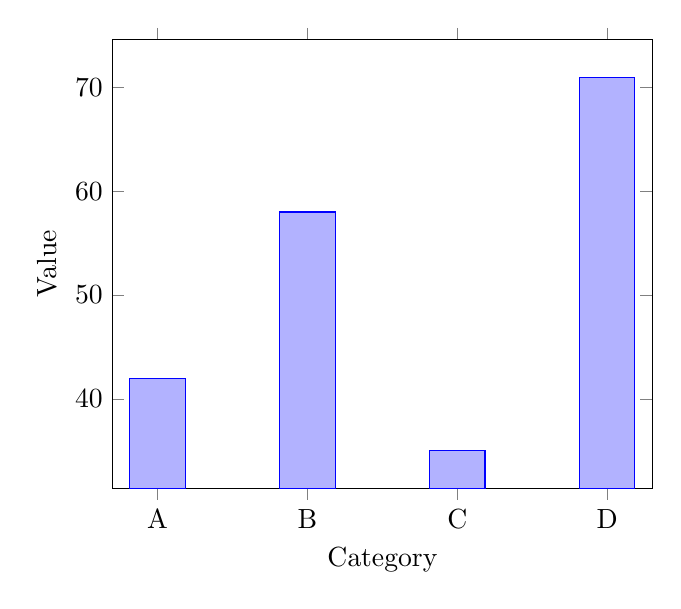
\begin{tikzpicture}
    \begin{axis}[
        ybar,
        xlabel={Category},
        ylabel={Value},
        symbolic x coords={A, B, C, D},
        xtick=data,
        bar width=20pt,
    ]
        \addplot coordinates {(A,42) (B,58) (C,35) (D,71)};
    \end{axis}
\end{tikzpicture}
\end{verbatim}

For stacked bars:

\begin{verbatim}
\begin{axis}[
    ybar stacked,
    symbolic x coords={Q1, Q2, Q3, Q4},
    xtick=data,
]
    \addplot coordinates {(Q1,10) (Q2,15) (Q3,12) (Q4,20)};
    \addplot coordinates {(Q1,8)  (Q2,9)  (Q3,14) (Q4,11)};
    \legend{Series A, Series B}
\end{axis}
\end{verbatim}

\section{Contour Plots}

Contour plots require \texttt{gnuplot} as a backend. Ensure gnuplot is
installed and pass \texttt{-{}-shell-escape} to the \LaTeX{} engine:

\begin{verbatim}
\begin{tikzpicture}
    \begin{axis}[
        view={0}{90},
        colorbar,
        title={Contour of $f(x,y) = x^2 - y^2$},
    ]
        \addplot3[
            contour gnuplot={levels={-4,-2,0,2,4}},
            domain=-2:2, domain y=-2:2,
            samples=30,
        ] {x^2 - y^2};
    \end{axis}
\end{tikzpicture}
\end{verbatim}

Custom functions replace the expression in braces. The \texttt{levels} key
controls which contour lines are drawn. Layer management allows combining
contour fills with surface plots by adjusting the \texttt{z buffer} order.

\section{Date Plots}

The \texttt{dateplot} library provides axis formatting for ISO 8601 dates:

\begin{verbatim}
\usepackage{pgfplots}
\usepgfplotslibrary{dateplot}

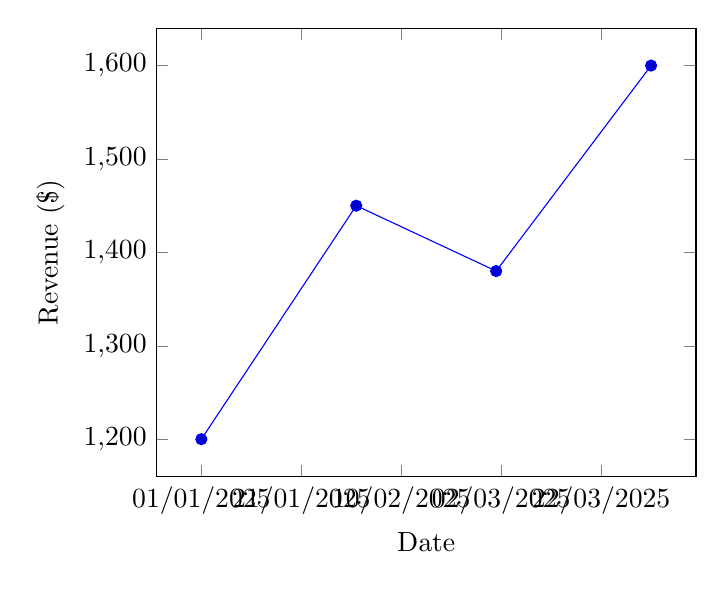
\begin{tikzpicture}
    \begin{axis}[
        date coordinates in=x,
        xticklabel={\day/\month/\year},
        xlabel={Date},
        ylabel={Revenue (\$)},
    ]
        \addplot coordinates {
            (2025-01-01, 1200)
            (2025-02-01, 1450)
            (2025-03-01, 1380)
            (2025-04-01, 1600)
        };
    \end{axis}
\end{tikzpicture}
\end{verbatim}

Date strings must follow the \texttt{YYYY-MM-DD} format. Use
\texttt{xticklabel} to customise the display format.

\section{CSV Data Import}

PGFPlots reads CSV files with \verb|\pgfplotstableread|:

\begin{verbatim}
\pgfplotstableread{data/measurements.csv}\datatable
\begin{tikzpicture}
    \begin{axis}[
        regularplot,
        xlabel={Time (s)},
        ylabel={Displacement (mm)},
    ]
        \addplot table [x=time, y=displacement] {\datatable};
    \end{axis}
\end{tikzpicture}
\end{verbatim}

Error bars are added with the \texttt{error bars/.cd} keys:

\begin{verbatim}
\addplot[
    table[x=time, y=displacement, y error=uncertainty],
    error bars/.cd, y dir=both, y explicit,
] {\datatable};
\end{verbatim}

Filter rows with \verb|\pgfplotsinvokeforeach| or the \texttt{skip coords
between index} key. Column selection uses \texttt{x=colname} and
\texttt{y=colname} to pick arbitrary columns from the data table.

\section{Custom Styles}

OmniLaTeX defines several PGFPlots styles and color cycles:

\begin{longtblr}[
    caption = {OmniLaTeX PGFPlots styles},
    label = {tab:pgfplots-styles},
]{colspec = {l l}, rowhead = 1}
    \toprule
    Style / Cycle  & Description \\
    \midrule
    regularplot    & Default: grid lines, axis box, mark size 2pt \\
    plainplot      & No grid, no box, minimal frame \\
    tuftelike      & Tufte aesthetic: thin grid, no box, data-ink focus \\
    arrowplot      & Arrow markers at each data point \\
    RdYlBu3        & Diverging colour cycle: red--yellow--blue \\
    mod mark list  & Alternating mark styles for multi-series plots \\
    viridis        & Perceptually uniform colour cycle \\
    \bottomrule
\end{longtblr}

Select a colour cycle with the \texttt{cycle list name} key:

\begin{verbatim}
\begin{axis}[
    regularplot,
    cycle list name=viridis,
]
    \addplot coordinates { ... };
    \addplot coordinates { ... };
\end{axis}
\end{verbatim}

\section{Dual Axes}

Add a secondary y-axis using \texttt{axis y line*=right} on a second
\texttt{axis} environment:

\begin{verbatim}
\begin{tikzpicture}
    \begin{axis}[
        regularplot,
        axis y line*=left,
        xlabel={Time (s)},
        ylabel={Temperature (K)},
    ]
        \addplot coordinates { (0,293) (5,325) };
    \end{axis}
    \begin{axis}[
        regularplot,
        axis y line*=right,
        axis x line=none,
        ylabel={Pressure (kPa)},
        ylabel style={at={(1,0.5)}},
    ]
        \addplot coordinates { (0,101) (5,115) };
    \end{axis}
\end{tikzpicture}
\end{verbatim}

The second axis hides its x-axis with \texttt{axis x line=none} and positions
the y-label on the right with \texttt{ylabel style}.

\section{Groupplots}

The \texttt{groupplots} library arranges multiple plots in a grid with shared
axes:

\begin{verbatim}
\usepgfplotslibrary{groupplots}

\begin{tikzpicture}
    \begin{groupplot}[
        group style={
            group size=2 by 1,
            horizontal sep=2cm,
        },
        regularplot,
        width=0.45\textwidth,
    ]
        \nextgroupplot[title={Plot A}]
        \addplot coordinates { (0,1) (1,3) (2,2) };

        \nextgroupplot[title={Plot B}]
        \addplot coordinates { (0,4) (1,2) (2,5) };
    \end{groupplot}
\end{tikzpicture}
\end{verbatim}

\texttt{group size=columns by rows} sets the grid layout.
\texttt{horizontal sep} and \texttt{vertical sep} control spacing between
plots. Shared axis labels are set at the group level; per-plot overrides use
\texttt{\textbackslash nextgroupplot[...]}.
